\documentclass[./main.tex]{subfiles}
\graphicspath{{\subfix{./figs}}}

% ------------ main document ------------ 
\begin{document}

\chapter{Um capítulo mais complexo} \label{chap:2}
\thispagestyle{fancy}

\section{Uma seção básica} \label{chp2:sec1}

\begin{adjustwidth}{\bodytab}{0mm}
\par Podemos estabelecer uma sigla \gls{ana}, e citar ela na forma curta \acrshort{ana} ou longa \acrlong{ana} consectetur adipiscing elit. Podemos citar uma referência \cite{descartes2008discurso}. A citação em linha pode ser customizada com vários estilos\footnote{Também é possível implementar notas de rodapé, como esta. Sed ac bibendum orci. Cras erat elit, consequat vel erat ac, tincidunt pulvinar. Curabitur at mollis eros. Integer ornare erat neque, id finibus velit ultrices in. Suspendisse dapibus tortor eget lorem pretium venenatis.}. Sed ac bibendum orci. Cras erat elit, consequat vel erat ac, tincidunt pulvinar\footnote{Quantas notas de rodapé forem necessárias, incluindo referências a outras seções como a Seção \ref{chp1:sec1:sub2}.}.. Curabitur at mollis eros. Integer ornare erat neque, id finibus velit ultrices in. Suspendisse dapibus tortor eget lorem pretium venenatis. Luctus accumsan tortor posuere ac ut consequat semper viverra. Mauris commodo quis imperdiet massa tincidunt nunc. Arcu odio ut sem nulla. Iaculis eu non diam phasellus vestibulum lorem sed. Vitae tortor condimentum lacinia quis vel eros donec ac odio. 

\subsection{Esta é uma subseção} \label{chp2:sec1:sub1}

\par Est sit amet facilisis magna etiam tempor. Luctus accumsan tortor posuere ac ut consequat semper viverra. Mauris commodo quis imperdiet massa tincidunt nunc. Arcu odio ut sem nulla. Iaculis eu non diam phasellus vestibulum lorem sed. Vitae tortor condimentum lacinia quis vel eros donec ac odio. Ornare arcu dui vivamus arcu. Nibh tellus molestie nunc non. Et netus et malesuada fames ac turpis egestas sed tempus. Eleifend donec pretium vulputate sapien nec. Sed lectus vestibulum mattis ullamcorper. Tincidunt dui ut ornare lectus sit. Donec adipiscing tristique risus nec feugiat in fermentum posuere urna. Ultricies lacus sed turpis tincidunt id aliquet risus feugiat. Ac placerat vestibulum lectus mauris ultrices eros in. Consectetur a erat nam at lectus urna. Enim neque volutpat ac tincidunt vitae semper quis lectus nulla. Feugiat sed lectus vestibulum mattis ullamcorper.

\par Est sit amet facilisis magna etiam tempor. Luctus accumsan tortor posuere ac ut consequat semper viverra. Mauris commodo quis imperdiet massa tincidunt nunc. Arcu odio ut sem nulla. Iaculis eu non diam phasellus vestibulum lorem sed. Vitae tortor condimentum lacinia quis vel eros donec ac odio. Ornare arcu dui vivamus arcu. Nibh tellus molestie nunc non. Et netus et malesuada fames ac turpis egestas sed tempus. Eleifend donec pretium vulputate sapien nec. Sed lectus vestibulum mattis ullamcorper. Tincidunt dui ut ornare lectus sit. Donec adipiscing tristique risus nec feugiat in fermentum posuere urna. Ultricies lacus sed turpis tincidunt id aliquet risus feugiat. Ac placerat vestibulum lectus mauris ultrices eros in. Consectetur a erat nam at lectus urna. Enim neque volutpat ac tincidunt vitae semper quis lectus nulla. Feugiat sed lectus vestibulum mattis ullamcorper.

\subsection{Esta é outra subseção}  \label{chp2:sec1:sub2}

\par Est sit amet facilisis magna etiam tempor. Luctus accumsan tortor posuere ac ut consequat semper viverra. Mauris commodo quis imperdiet massa tincidunt nunc. Arcu odio ut sem nulla. Iaculis eu non diam phasellus vestibulum lorem sed. Vitae tortor condimentum lacinia quis vel eros donec ac odio. Ornare arcu dui vivamus arcu. Nibh tellus molestie nunc non. Et netus et malesuada fames ac turpis egestas sed tempus. Eleifend donec pretium vulputate sapien nec. Sed lectus vestibulum mattis ullamcorper. Tincidunt dui ut ornare lectus sit. Donec adipiscing tristique risus nec feugiat in fermentum posuere urna. Ultricies lacus sed turpis tincidunt id aliquet risus feugiat. Ac placerat vestibulum lectus mauris ultrices eros in. Consectetur a erat nam at lectus urna. Enim neque volutpat ac tincidunt vitae semper quis lectus nulla. Feugiat sed lectus vestibulum mattis ullamcorper.

\subsection{Aqui temos uma figura grande}  \label{chp2:sec1:sub3}

\begin{figure}[t!] % place figure in the page
	\centering                                       
	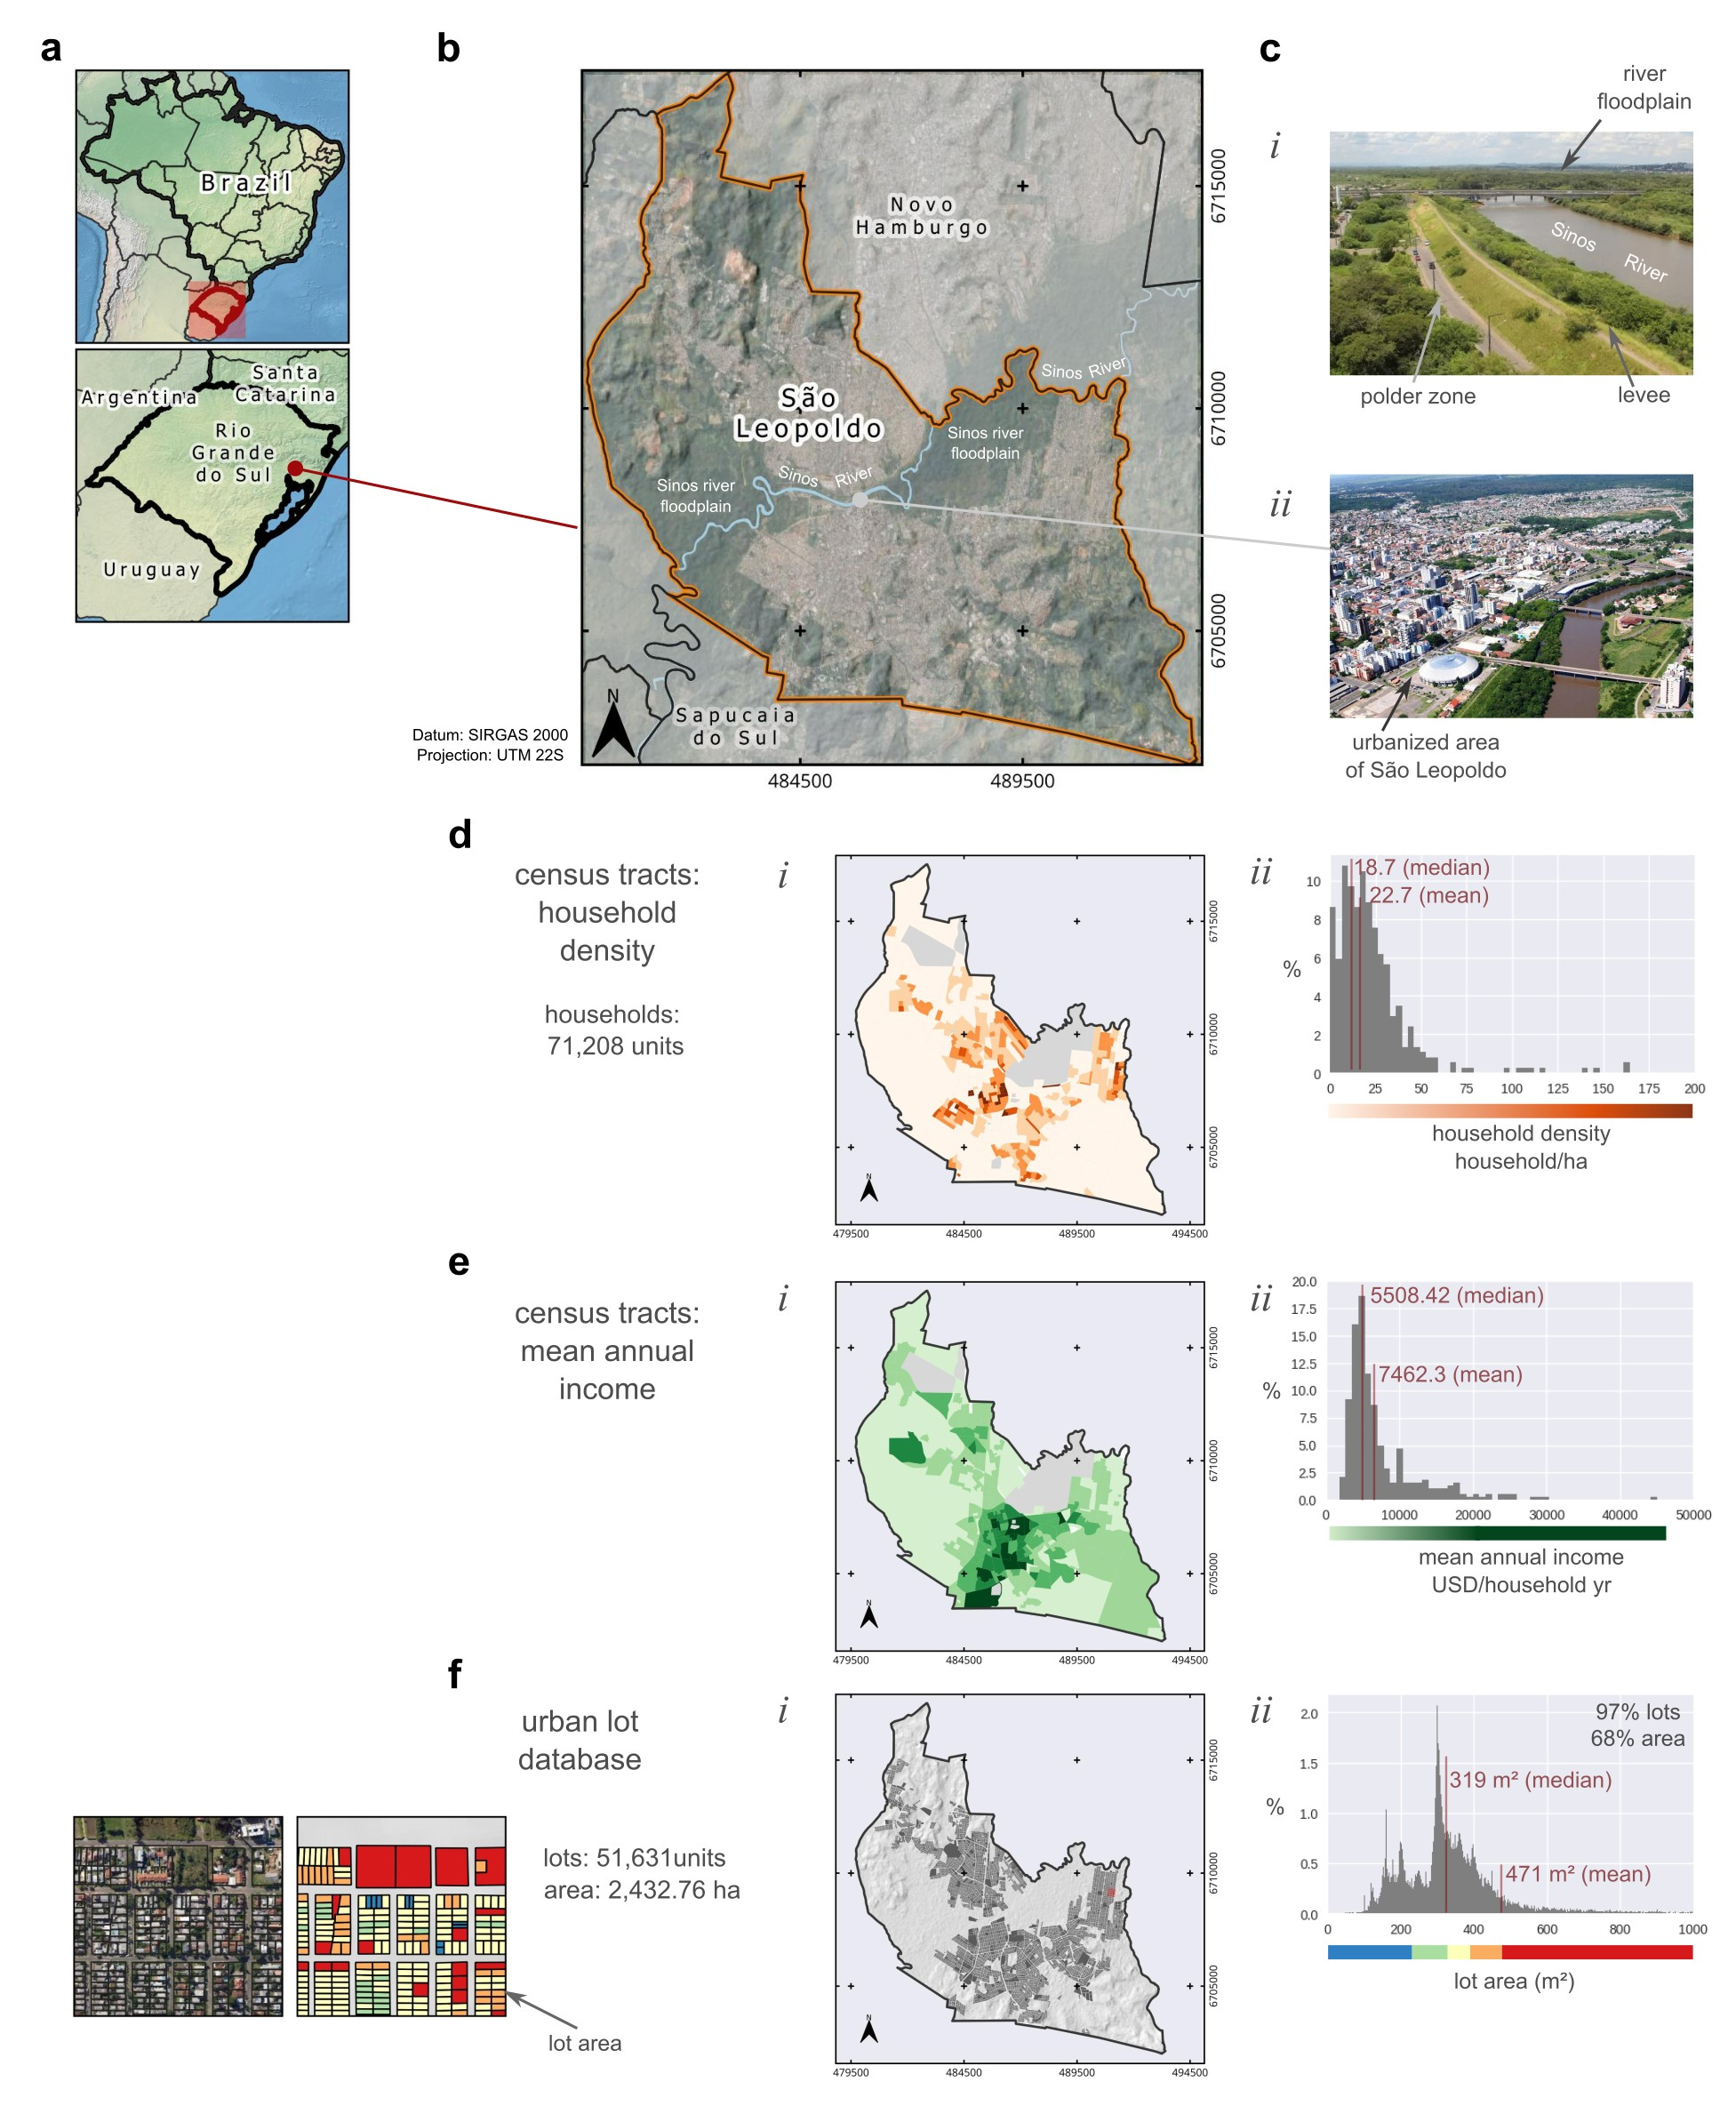
\includegraphics[width=0.98\linewidth]{figs/fig_case.jpg}    
	\caption[Curabitur at mollis eros]
	{\textbf{---\;Et netus et malesuada fames ac turpis egestas sed tempus}.
		\textbf{a}\,--\,Curabitur at mollis eros. Integer ornare erat neque, id finibus velit ultrices in. Suspendisse dapibus tortor eget lorem pretium venenatis (detail \textrm{\textit{i}}); Cras erat elit, consequat vel erat ac, tincidunt pulvinar. Curabitur at mollis eros. Integer ornare erat neque, id finibus velit ultrices in (detail \textrm{\textit{ii}}).
		\textbf{b}\,--\,Cras erat elit, consequat vel erat ac, tincidunt pulvinar. Curabitur at mollis eros. Integer ornare erat neque, id finibus velit ultrices in (detail \textrm{\textit{i}}); Cras erat elit, consequat vel erat ac, tincidunt pulvinar. Curabitur at mollis eros. Integer ornare erat neque, id finibus velit ultrices in (detail \textrm{\textit{ii}}).
          \textbf{c}\,--\,Suspendisse dapibus tortor eget lorem pretium venenatis (detail \textrm{\textit{i}}); Cras erat elit, consequat vel erat ac, tincidunt pulvinar. Curabitur at mollis eros. Integer ornare erat neque, id finibus velit ultrices in (detail \textrm{\textit{ii}}).
	}
	\label{fig:fig_large}  % use qualitative label                      
\end{figure}

\par A Figura \ref{fig:fig_large} pode ser citada em qualquer parte do texto. Est sit amet facilisis magna etiam tempor. Luctus accumsan tortor posuere ac ut consequat semper viverra. Mauris commodo quis imperdiet massa tincidunt nunc. Arcu odio ut sem nulla. Iaculis eu non diam phasellus vestibulum lorem sed. Vitae tortor condimentum lacinia quis vel eros donec ac odio. Ornare arcu dui vivamus arcu. Nibh tellus molestie nunc non. Et netus et malesuada fames ac turpis egestas sed tempus. Eleifend donec pretium vulputate sapien nec. Sed lectus vestibulum mattis ullamcorper. Tincidunt dui ut ornare lectus sit. Donec adipiscing tristique risus nec feugiat in fermentum posuere urna. Ultricies lacus sed turpis tincidunt id aliquet risus feugiat. Ac placerat vestibulum lectus mauris ultrices eros in. Consectetur a erat nam at lectus urna. Enim neque volutpat ac tincidunt vitae semper quis lectus nulla. Feugiat sed lectus vestibulum mattis ullamcorper.

\par Est sit amet facilisis magna etiam tempor. Luctus accumsan tortor posuere ac ut consequat semper viverra. Mauris commodo quis imperdiet massa tincidunt nunc. Arcu odio ut sem nulla. Iaculis eu non diam phasellus vestibulum lorem sed. Vitae tortor condimentum lacinia quis vel eros donec ac odio. Ornare arcu dui vivamus arcu. Nibh tellus molestie nunc non. Et netus et malesuada fames ac turpis egestas sed tempus. Eleifend donec pretium vulputate sapien nec. Sed lectus vestibulum mattis ullamcorper. Tincidunt dui ut ornare lectus sit. Donec adipiscing tristique risus nec feugiat in fermentum posuere urna. Ultricies lacus sed turpis tincidunt id aliquet risus feugiat. Ac placerat vestibulum lectus mauris ultrices eros in. Consectetur a erat nam at lectus urna. Enim neque volutpat ac tincidunt vitae semper quis lectus nulla. Feugiat sed lectus vestibulum mattis ullamcorper. Nibh tellus molestie nunc non. Et netus et malesuada fames ac turpis egestas sed tempus. Eleifend donec pretium vulputate sapien nec. Sed lectus vestibulum mattis ullamcorper. Tincidunt dui ut ornare lectus sit. Donec adipiscing tristique risus nec feugiat in fermentum posuere urna. Ultricies lacus sed turpis tincidunt id aliquet risus feugiat. Ac placerat vestibulum lectus mauris ultrices eros in. Consectetur a erat nam at lectus urna. Enim neque volutpat ac tincidunt vitae semper quis lectus nulla. Feugiat sed lectus vestibulum mattis ullamcorper.
\end{adjustwidth}


\section{Uma nova seção} \label{chp2:sec2}

\begin{adjustwidth}{\bodytab}{0mm}

\par Est sit amet facilisis magna etiam tempor. Luctus accumsan tortor posuere ac ut consequat semper viverra. Mauris commodo quis imperdiet massa tincidunt nunc. Arcu odio ut sem nulla. Iaculis eu non diam phasellus vestibulum lorem sed. Vitae tortor condimentum lacinia quis vel eros donec ac odio. Ornare arcu dui vivamus arcu. Nibh tellus molestie nunc non. Et netus et malesuada fames ac turpis egestas sed tempus. Eleifend donec pretium vulputate sapien nec. Sed lectus vestibulum mattis ullamcorper. Tincidunt dui ut ornare lectus sit.

\subsection{Outra subseção} \label{chp2:sec2:sub1}

\blindtext[3]

\subsection{Aqui temos uma tabela bem grande}  \label{chp2:sec2:sub2}

\par A Tabela \ref{tab:actions_1} pode ser citada em qualquer parte. st sit amet facilisis magna etiam tempor. Luctus accumsan tortor posuere ac ut consequat semper viverra. Mauris commodo quis imperdiet massa tincidunt nunc. Arcu odio ut sem nulla. Iaculis eu non diam phasellus vestibulum lorem sed. Vitae tortor condimentum lacinia quis vel eros donec ac odio. Ornare arcu dui vivamus arcu. Nibh tellus molestie nunc non. Et netus et malesuada fames ac turpis egestas sed tempus. Eleifend donec pretium vulputate sapien nec. Sed lectus vestibulum mattis ullamcorper. Tincidunt dui ut ornare lectus sit. Donec adipiscing tristique risus nec feugiat in fermentum posuere urna. Ultricies lacus sed turpis tincidunt id aliquet risus feugiat. Ac placerat vestibulum lectus mauris ultrices eros in. Consectetur a erat nam at lectus urna. Enim neque volutpat ac tincidunt vitae semper quis lectus nulla. Feugiat sed lectus vestibulum mattis ullamcorper.


\begin{table}[t]
    \centering
    \tiny
    \rowcolors{2}{white}{rowgray}
\begin{tabular}{lllllrrr}
\toprule
\textbf{Action Code} &          \textbf{Type}&   \textbf{Urgency} &   \textbf{Subsystem} &                \textbf{Zone} &  \textbf{Start} &  \textbf{End} &    \textbf{$P_k$ (USD million)} \\
\midrule
 a.3 &   Maintenance & Immediate & Channels &           Municipal &   2023 & 2036 & 63.02 \\
 a.1 &     Expansion &       Low &   Polder &           Municipal &   2023 & 2030 & 38.53 \\
a.56 &     Expansion &       Low &   Polder & Subcat. João Corrêa &   2023 & 2030 & 32.59 \\
 a.5 &   Maintenance & Immediate &   Sewers &           Municipal &   2023 & 2036 & 25.82 \\
a.68 &     Expansion &  Moderate &   Polder &   Subcat. Cerquinha &   2027 & 2036 & 19.46 \\
a.16 &     Operation &       Low & Channels &           Municipal &   2023 & 2036 & 10.47 \\
a.15 &     Operation & Immediate &   Polder &           Municipal &   2023 & 2036 &  9.67 \\
a.69 &     Expansion & Immediate & Channels &   Subcat. Cerquinha &   2023 & 2033 &  7.68 \\
 a.4 & Rehabilitaion &      High & Channels &           Municipal &   2023 & 2028 &  7.50 \\
 a.6 &   Maintenance &      High & Channels &           Municipal &   2023 & 2036 &  6.65 \\
 a.2 &   Maintenance &      High &   Polder &           Municipal &   2023 & 2036 &  6.36 \\
a.45 &     Expansion &  Moderate & Channels & Subcat. João Corrêa &   2027 & 2036 &  4.23 \\
a.51 &     Expansion &  Moderate & Channels & Subcat. João Corrêa &   2027 & 2036 &  4.00 \\
a.53 &     Expansion & Immediate &   Polder & Subcat. João Corrêa &   2023 & 2033 &  3.74 \\
a.14 &     Operation & Immediate &   Polder &           Municipal &   2023 & 2036 &  3.43 \\
a.11 &     Operation & Immediate &   Sewers &           Municipal &   2023 & 2036 &  3.03 \\
a.66 &     Expansion & Immediate &   Polder &   Subcat. Cerquinha &   2023 & 2033 &  2.89 \\
a.26 &     Expansion &      High & Channels &  Subcat. Sem Nome I &   2025 & 2028 &  2.87 \\
a.55 &     Expansion &      High & Channels & Subcat. João Corrêa &   2025 & 2028 &  2.86 \\
a.59 &     Expansion &      High & Channels &   Subcat. Gauchinho &   2025 & 2028 &  2.08 \\
a.28 &     Expansion &  Moderate & Channels &    Subcat. Quilombo &   2027 & 2036 &  1.99 \\
a.10 &     Operation & Immediate &   Sewers &           Municipal &   2023 & 2036 &  1.83 \\
a.54 &     Expansion & Immediate &   Polder & Subcat. João Corrêa &   2023 & 2033 &  1.63 \\
a.38 &     Expansion &  Moderate & Channels &       Subcat. Kruse &   2027 & 2036 &  1.24 \\
 a.7 &     Expansion &  Moderate &   Polder &           Municipal &   2027 & 2036 &  1.12 \\
a.57 &     Expansion &  Moderate & Channels & Subcat. João Corrêa &   2027 & 2036 &  1.11 \\
a.41 &     Expansion &  Moderate & Channels &       Subcat. Kruse &   2027 & 2036 &  1.09 \\
a.58 &     Expansion &      High & Channels &   Subcat. Gauchinho &   2025 & 2028 &  1.03 \\
a.67 &     Expansion &  Moderate & Channels &   Subcat. Cerquinha &   2027 & 2036 &  0.89 \\
a.50 &     Expansion &  Moderate & Channels & Subcat. João Corrêa &   2027 & 2036 &  0.81 \\
a.24 &     Expansion &  Moderate & Channels & Subcat. Sem Nome II &   2027 & 2036 &  0.77 \\
 a.8 & Rehabilitaion & Immediate &   Polder &           Municipal &   2023 & 2030 &  0.76 \\
a.42 &     Expansion &  Moderate & Channels &       Subcat. Kruse &   2027 & 2036 &  0.71 \\
a.37 &     Expansion &  Moderate & Channels &       Subcat. Kruse &   2027 & 2036 &  0.68 \\
a.48 &     Expansion &  Moderate & Channels & Subcat. João Corrêa &   2027 & 2036 &  0.64 \\
\bottomrule
\end{tabular}
\caption[Uma Tabela bem grande]{\textbf{(first part)} List of planned actions for stormwater derived from the São Leopoldo's Urban Stormwater and Flood Protection master plan. Note: $P_k$ is the present worth (2023) for the estimated action cost.}
\label{tab:actions_1}
\end{table}

\begin{table}[h]
    \centering
    \tiny
    \rowcolors{2}{white}{rowgray}
\begin{tabular}{lllllrrr}
\toprule
\textbf{Action Code} &          \textbf{Type}&   \textbf{Urgency} &   \textbf{Subsystem} &                \textbf{Zone} &  \textbf{Start} &  \textbf{End} &    \textbf{$P_k$ (USD million)} \\
\midrule
a.43 &     Expansion &  Moderate & Channels &       Subcat. Kruse &   2027 & 2036 &  0.61 \\
a.27 &     Expansion &  Moderate & Channels &    Subcat. Quilombo &   2027 & 2036 &  0.58 \\
a.64 &     Expansion &  Moderate & Channels &   Subcat. Cerquinha &   2027 & 2036 &  0.58 \\
a.40 &     Expansion &  Moderate & Channels &       Subcat. Kruse &   2027 & 2036 &  0.53 \\
a.49 &     Expansion &  Moderate & Channels & Subcat. João Corrêa &   2027 & 2036 &  0.52 \\
a.46 &     Expansion &  Moderate & Channels & Subcat. João Corrêa &   2027 & 2036 &  0.51 \\
a.44 &     Expansion &  Moderate & Channels &       Subcat. Kruse &   2027 & 2036 &  0.39 \\
a.62 &     Expansion &  Moderate & Channels &   Subcat. Cerquinha &   2027 & 2036 &  0.39 \\
a.52 &     Expansion &  Moderate & Channels & Subcat. João Corrêa &   2027 & 2036 &  0.35 \\
 a.9 & Rehabilitaion &      High &   Polder &           Municipal &   2025 & 2028 &  0.30 \\
a.21 &     Expansion &  Moderate & Channels &       Baixo Sino 36 &   2027 & 2036 &  0.29 \\
a.12 &     Operation &      High &   Polder &           Municipal &   2023 & 2036 &  0.27 \\
a.20 &     Expansion &  Moderate & Channels &       Baixo Sino 36 &   2027 & 2036 &  0.26 \\
a.39 &     Expansion &  Moderate & Channels &       Subcat. Kruse &   2027 & 2036 &  0.26 \\
a.65 &     Expansion &  Moderate &   Sewers &   Subcat. Cerquinha &   2027 & 2036 &  0.24 \\
a.18 &     Expansion &  Moderate & Channels &       Baixo Sino 37 &   2027 & 2036 &  0.18 \\
a.22 &     Expansion &  Moderate &   Sewers & Subcat. Sem Nome II &   2027 & 2036 &  0.17 \\
a.19 &     Expansion &  Moderate & Channels &       Baixo Sino 37 &   2027 & 2036 &  0.12 \\
a.25 &     Expansion &  Moderate & Channels & Subcat. Sem Nome II &   2027 & 2036 &  0.09 \\
a.17 &   Maintenance & Immediate &   Polder & Subcat. João Corrêa &   2023 & 2036 &  0.09 \\
a.31 &     Expansion &  Moderate & Channels &    Subcat. Manteiga &   2027 & 2036 &  0.08 \\
a.60 &     Expansion &  Moderate & Channels &   Subcat. Cerquinha &   2027 & 2036 &  0.07 \\
a.29 &     Expansion &  Moderate & Channels &    Subcat. Manteiga &   2027 & 2036 &  0.07 \\
a.32 &     Expansion &  Moderate & Channels &    Subcat. Manteiga &   2027 & 2036 &  0.07 \\
a.70 &     Expansion &  Moderate & Channels &        Subcat. Bopp &   2027 & 2036 &  0.07 \\
a.63 &     Expansion &  Moderate & Channels &   Subcat. Cerquinha &   2027 & 2036 &  0.06 \\
a.61 &     Expansion &  Moderate & Channels &   Subcat. Cerquinha &   2027 & 2036 &  0.05 \\
a.34 &     Expansion &  Moderate & Channels &       Subcat. Kruse &   2027 & 2036 &  0.05 \\
a.33 &     Expansion &  Moderate & Channels &    Subcat. Manteiga &   2027 & 2036 &  0.03 \\
a.35 &     Expansion &  Moderate & Channels &       Subcat. Kruse &   2027 & 2036 &  0.03 \\
a.30 &     Expansion &  Moderate & Channels &    Subcat. Manteiga &   2027 & 2036 &  0.03 \\
a.23 &     Expansion &  Moderate & Channels & Subcat. Sem Nome II &   2027 & 2036 &  0.02 \\
a.36 &     Expansion &  Moderate & Channels &       Subcat. Kruse &   2027 & 2036 &  0.02 \\
a.47 &     Expansion &  Moderate &   Sewers & Subcat. João Corrêa &   2027 & 2036 &  0.02 \\
a.71 &     Expansion &  Moderate & Channels &        Subcat. Bopp &   2027 & 2036 &  0.01 \\
a.13 &     Operation &  Moderate &   Polder &           Municipal &   2027 & 2036 &  0.01 \\
\bottomrule
\end{tabular}
\caption*{\textbf{Table \ref{tab:actions_1} (continued)} List of planned actions for stormwater derived from the São Leopoldo's Urban Stormwater and Flood Protection master plan. Note: $P_k$ is the present worth (2023) for the estimated action cost.}
\end{table}

\blindtext[2]

\blindtext[2]

\end{adjustwidth}


\section{A última seção} \label{chp2:sec3}

\begin{adjustwidth}{\bodytab}{0mm}

\par Est sit amet facilisis magna etiam tempor. Luctus accumsan tortor posuere ac ut consequat semper viverra. Mauris commodo quis imperdiet massa tincidunt nunc. Arcu odio ut sem nulla. Iaculis eu non diam phasellus vestibulum lorem sed. Vitae tortor condimentum lacinia quis vel eros donec ac odio.

\blindtext[2]

\subsection{Aqui temos um destaque} \label{chp2:sec3:sub1}

\blindtext[2]

\begin{simplebox}[
    width=140mm,
    float=t,
    label={destaque_curvas_chave},
    nameref={Curvas-chave}
    ]{Bandas de incerteza de vazão a partir de curvas-chave}
    \footnotesize
    % first minipage
    \begin{minipage}[t]{\linewidth}    
    \par A \textbf{vazão} em rios quase nunca é medida diretamente, pois para isso é preciso uma equipe técnica especializada. É muito mais fácil e barato observar o \textbf{nível} dos rios a partir de réguas linimétricas. De fato, o nível de muitos rios no Brasil é observado duas vezes ao dia em estações fluviométricas da Rede Hidrometeorológica Nacional. Assim, as raras observações de vazão factíveis são utilizadas na construção de uma \textbf{curvas-chave}, que geralmente é um modelo matemático do tipo potência:
    \begin{equation*} % the equation environment. 
    		\label{eq:rating_curve}
    		Q = a \cdot (h - h_0)^b
    \end{equation*}
    Em que $Q$ é a vazão em $m^{3}/s$; $h$ é o nível observado, e; $h_0$, $a$ e $b$ são os parâmetros do modelo. Essa curva pode então ser usada para a estimativa da vazão a partir das observações rotineiras de nível. 
    \end{minipage}
    % second min
    \begin{minipage}[t]{\linewidth}
        \begin{minipage}[t]{\linewidth}
        \vspace*{5pt}
        	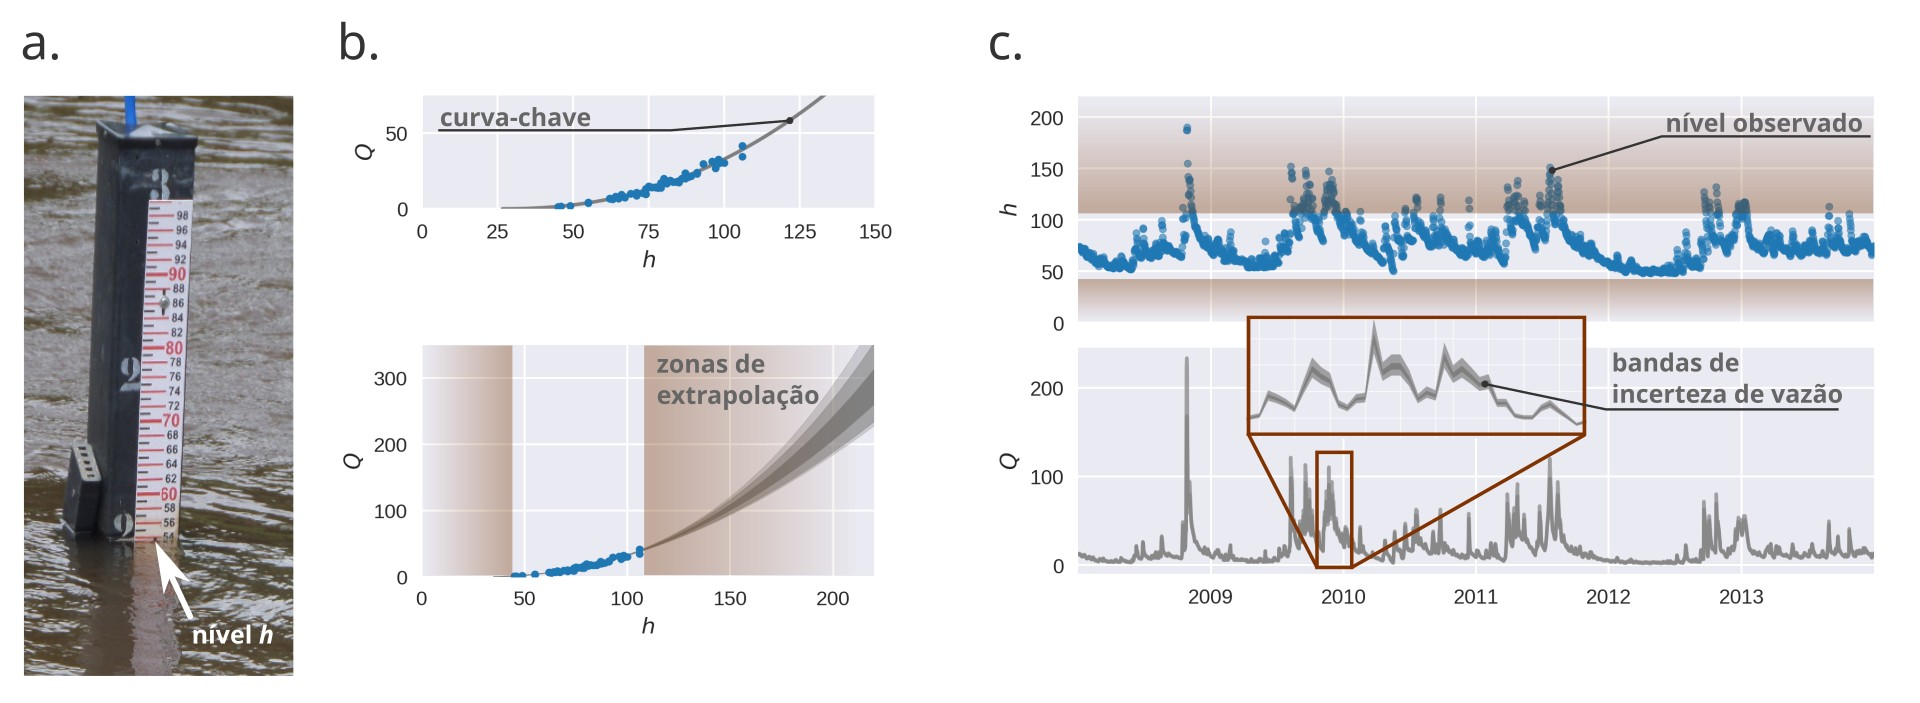
\includegraphics[width=\linewidth]{fig_ratingcurve.jpg}		
        	\captionof{figure}[Bandas de incerteza de vazão a partir de curvas-chave]{
                \textbf{---\;Bandas de incerteza de vazão a partir de curvas-chave.}\;\textbf{a.}---\;Observação de nível $h$ em uma régua linimétrica.\;\textbf{b.}---\;Ajuste de um modelo tipo potência e estimativa da incerteza por métodos de reamostragem do erro.\;\textbf{c.}---\;Série histórica de nível e bandas de incerteza da vazão.
        	}
            \label{fig:rating-curve}  % use qualitative label	
        \vspace*{5pt}
    \end{minipage}
    % next
    \end{minipage}
    \begin{minipage}[t]{\linewidth}
    \par Como ilustrado na Figura \ref{fig:rating-curve}, a confirmação desse modelo diante das evidências de nível e vazão inicia-se por ajustar os parâmetros aos dados disponíveis com técnicas de otimização. O comportamento do erro aleatório pode ser então avaliado. A variância do erro, se estabilizada, permite reamostragens estatisticamente equivalentes dos dados (simulações de Monte Carlo). As bandas de incerteza da curva-chave, assim, se refletem na incerteza da estimativa na série histórica de vazão. No exemplo apresentado, nota-se que existem \textbf{zonas de extrapolação} nos extremos, onde a incerteza se expande desproporcionalmente.    
    \end{minipage}
\label{box:rating-curve}
\normalsize
\end{simplebox}

\blindtext[2]

\end{adjustwidth}


\section{Recomendações} \label{chp2:summary}

\begin{adjustwidth}{\bodytab}{0mm}
\par Geralmente é legal terminar um capítulo com recomendações. Est sit amet facilisis magna etiam tempor. Luctus accumsan tortor posuere ac ut consequat semper viverra. Mauris commodo quis imperdiet massa tincidunt nunc. Arcu odio ut sem nulla. Iaculis eu non diam phasellus vestibulum lorem sed. Vitae tortor condimentum lacinia quis vel eros donec ac odio. Ornare arcu dui vivamus arcu. Nibh tellus molestie nunc non.

\begin{itemize}
    \item[$\blacksquare$] \textbf{Primeira recomendação}. Est sit amet facilisis magna etiam tempor. Luctus accumsan tortor posuere ac ut consequat semper viverra. Mauris commodo quis imperdiet massa tincidunt nunc. Arcu odio ut sem nulla. Iaculis eu non diam phasellus vestibulum lorem sed. Vitae tortor condimentum lacinia quis vel eros donec ac odio. Ornare arcu dui vivamus arcu. Nibh tellus molestie nunc non.
    \item  [$\blacksquare$] \textbf{Segunda recomendação}. Est sit amet facilisis magna etiam tempor. Luctus accumsan tortor posuere ac ut consequat semper viverra. Mauris commodo quis imperdiet massa tincidunt nunc. Arcu odio ut sem nulla. Iaculis eu non diam phasellus vestibulum lorem sed. Vitae tortor condimentum lacinia quis vel eros donec ac odio. Ornare arcu dui vivamus arcu. Nibh tellus molestie nunc non.
    \item[$\blacksquare$] \textbf{Terceira recomendação}.Est sit amet facilisis magna etiam tempor. Luctus accumsan tortor posuere ac ut consequat semper viverra. Mauris commodo quis imperdiet massa tincidunt nunc. Arcu odio ut sem nulla. Iaculis eu non diam phasellus vestibulum lorem sed. Vitae tortor condimentum lacinia quis vel eros donec ac odio. Ornare arcu dui vivamus arcu. Nibh tellus molestie nunc non. 
\end{itemize}

\end{adjustwidth}


\end{document}
 